\section{Funzionamento}
Nella seguente sezione si descrive il funzionamento del veicolo, degli algoritmi utilizzati e delle scelte progettuali.

\subsection{Stack di guida autonoma}
La prima cosa da analizzare è il funzionamento dello stack di guida autonoma.
Lo stack funziona grazie a diversi processi, divisi (come descritto nell'introduzione) in perception, planning e control, di seguito una breve censita dei nodi ROS che permettono tale funzionamento:
Per quanto riguarda la parte di perception, vediamo due aspetti, i sensori e l'algoritmo di localizzazione:

\begin{itemize}
  \item \textbf{urg\_node}: È il nodo che permette di pubblicare sul topic ROS \textit{/scan} le pointcloud rilevate dal sensore Lidar, il tipo di dato utilizzato è chiamato \textit{LaserScan} e fornisce una serie di distanze che vanno insieme a formare ciò che il sensore Lidar rileva.
  \item \textbf{hunter\_ros2\_node}: Fornisce un interfaccia con il robot stesso, da questo nodo possiamo ricevere l'odometria calcolata a partire dal movimento delle ruote e, come vedremo successivamente, potremo pubblicare i comandi che il robot dovrà svolgere. Quello che interessa a noi al momento della perception è l'odometria del mezzo, che viene pubblicata sul tpoic \textit{/odometry} sottoforma di dato \textit{Odomentry}. 
  \item \textbf{particle\_filter}: Implementa l'algoritmo di localizzazione chiamato particle filter, questo algoritmo sfrutta per il suo funzionamento la mappa dell'ambiente in cui il robot si sta muovendo, l'odometria del veicolo e la pointcloud del sensore Lidar. Questo nodo pubblica la posizione calcolata sul topic ROS \textit{/pf/position} sottoforma di dato \textit{Odometry}.
\end{itemize}

\noindent Passando invece al momento del planning ci si avvale di due nodi:

\begin{itemize}
  \item \textbf{path\_logger}: Permette la registrazione di un percorso quando il veicolo viene guidato manualmentequesto percorso viene poi salvato in un file apposito.
  \item \textbf{path\_logger}: Questo nodo si occupa di pubblicare un percorso preregistrato o precalcolato da seguire, il dato è pubblicato sul topic \textit{/path}.  
\end{itemize}

\noindent Andiamo infine a descrivere il funzionamento della parte di controllo, questa è infatti composta da due nodi:

\begin{itemize}
  \item \textbf{purepursuit}: Si occupa di ricevere il percorso pubblicato sul topic \textit{/path} e a partire dalla posizione pubblicata dal nodo \textbf{particle\_filter} calcola i comandi da impartire al robot. I comandi vengono pubblicati sul topic\textit{/drive\_parameters} e sono di tipo \textit{Ackermann Stamped}, questo non è altro che un semplice tipo di messaggio ROS che incapsula il timestamp, un angolo di sterzo ed una velocità.
  \item \textbf{hunter\_ros2\_node}: Come descritto prima, questo nodo oltre a fornire l'odometria del mezzo, è anche capace di ricevere i comandi da impartire al robot. Il nodo è infatti in perenne ascolto sul topic \textit{/drive\_parameters} e ad ogni messaggio non farà altro che comunicare con l'interfaccia CAN del veicolo comunicandogli la velocità e l'angolo di sterzo da impostare.
\end{itemize}

\noindent di seguito uno schema riassuntivo di tutto il meccanismo:
\begin{figure}[h]
  \centering
  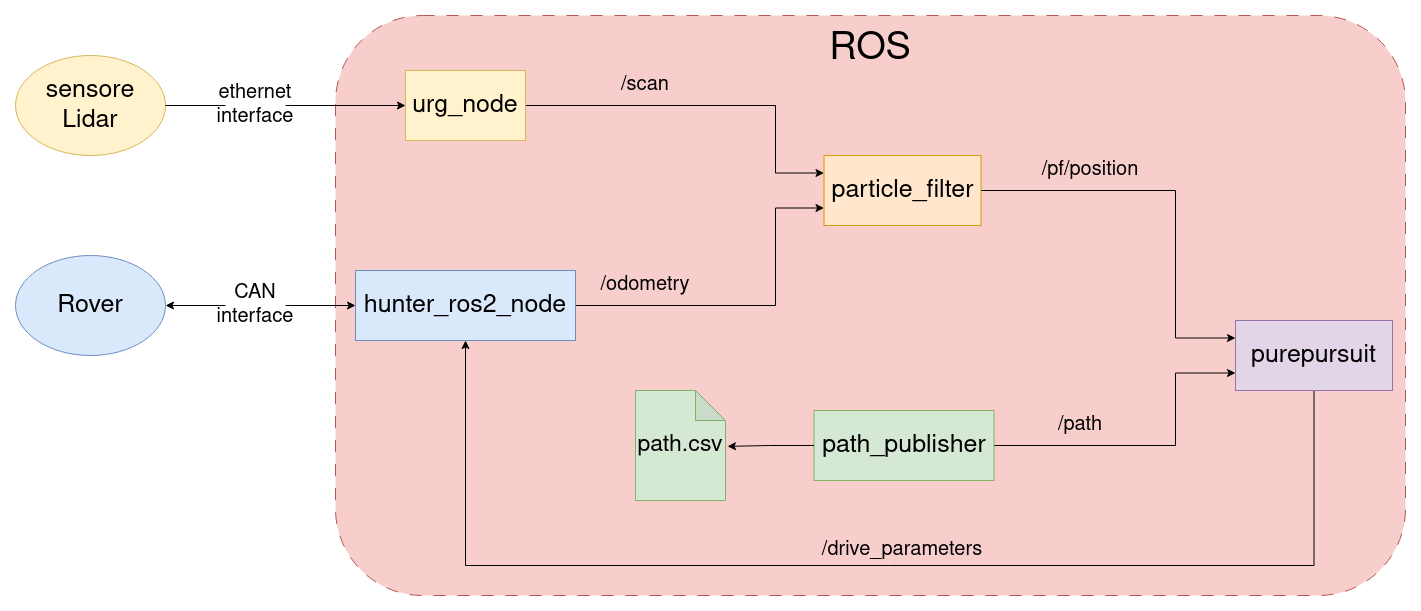
\includegraphics[width=1\textwidth]{figures/schema_guida_autonoma.png}
  \caption{Schema rissuntivo dello stack di guida autonoma}
  \label{Schema rissuntivo dello stack di guida autonoma}
\end{figure}

\subsection{guida remota}
Una volta illustrato e compreso il funzionamento dello stack di guida autonoma, è ora di passare alla pianificazione di quella remota.
La primissima domanda da porci è quale parte dello stack diventerà remoto, ad esempio si potrebbe decidere di svolgere solo la parte di planning da remoto e lasciare in resto in locale, o ad esempio di portare solo la perception. Si potrebbe anche decidere di far eseguire solo specifici nodi da remoto e lasciare in resto in locale.
\noindent Nella presente tesi si è scelto di portare in remoto quasi tutto lo stack, lasciando in locale solo i nodi che hanno strettamente bisogno dell'interfacciamento con l'hardare.

\noindent Nello specifico gli unici nodi che rimarranno in locale saranno:

\begin{itemize}
  \item \textbf{urg\_node}: Che sarà necessario per ricavare i dati dal sensore Lidar
  \item \textbf{hunter\_ros2\_node}: Necessario per ricavare l'odometria del mezzo e per inviare i comandi all'interfaccia CAN
\end{itemize}

\noindent Tutto il resto sarà gestito da remoto. Questo ci permette di poter scegliere con più flessibilità in quale modo pilotare il rover, si potrà infatti decidere sia di eseguire l'intero stack, senza modifiche, sulla macchina in remoto e di conseguenza inviare i comandi calcolati al mezzo, sia di poter guidare il veicolo completamente in manuale da un apposito operatore e di inviare solo i comandi scelti da quest'ultimo al veicolo.

\subsection{Nodi sviluppati}
Oltre ai nodi che già erano compresi nello stack di guida autonoma, è stato necessario sviluppare altri nodi che permettessero lo scambio di informazioni tra il veicolo e il server. Nello specifico i 3 nodi si iscriveranno a specifici topic ROS e pubblicheranno le stesse informazioni su topic MQTT.

\noindent Ogni nodo è diviso in più classi ed un unico main file, che gestirà l'intero flusso del nodo. All'interno del progetto che contiene il nodo sono anche compresi dei file di configurazione in formato yaml, dai quali il nodo andrà a leggere informazioni necessarie per l'esecuzione del processo.

\noindent È inoltre utile specificare che l'intera codebase è scritta in linguaggio c++, che risulta utile qualora sia necessario avere bassi tempi di esecuzione.

\subsubsection{MQTT telemery node}
La prima fase del progetto ha riguardato lo sviluppo di un componente software, ovvero un nodo ROS, in grado di interfacciarsi con i sensori del veicolo. Questo nodo, una volta configurato per sottoscriversi ai topic di interesse, è in grado di acquisire i dati provenienti dai sensori e di trasformarli in un formato adatto alla trasmissione. La scelta del formato JSON, ampiamente utilizzato per lo scambio di dati tra sistemi eterogenei, è stata dettata dalla sua leggibilità e dalla sua facilità di parsing. I dati, così formattati, vengono inviati al server MQTT.

\noindent I topic a cui il nodo effettua una subscribe sono:

\begin{itemize}
  \item \textit{/scan}: Per la ricezione della pointcloud rilevata dal sensore Lidar
  \item \textit{/odometry}: Per la ricezione dei dati di odometria del mezzo
\end{itemize}

\noindent Una volta ricevuto il dato, questo verrà formattato in una stringa JSON contente tutti i dati del messaggio. Una volta formattata, la stringa viene inserita all'interno di una cache, questa cache verrà poi inviata al server MQTT ad intervalli temporali regolari.

\noindent Un thread altro non è che un'unità di esecuzione parallela all'unità principale, chiamata main thread.

\noindent Il nodo è suddiviso in 6 classi:

\begin{itemize}
  \item \textbf{conf\_loader}: Si occupa di caricare i dati dai file di configurazione prima citati, nello specifico questa classe è stata implementata per rendere il main thread e il resto del processo indipendente dal formato dei file di configurazione.
  \item \textbf{mqtt\_publisher}: È una classe che contiene metodi utili all'invio di stringhe tramite protocollo MQTT e che si avvale della libreria paho.mqtt.cpp fornita dalla eclipse foundation. 
  \item \textbf{mqtt\_telemetry\_node}: Questa classe è quella che implementa il nodo ROS che si incaricherà di ricevere i dati utili alla telemetria.
  \item \textbf{msgs\_cache}: Questa classe implementa una semplice struttura dati che accoppia ad ogni topic ROS (rappresentata come stringa), una stringa JSON contente i dati di telemetria da inviare
  \item \textbf{msgs\_to\_string}: È un insieme di funzioni statiche che permette la traduzione da messaggi ROS a stringhe JSON
  \item \textbf{topic\_manager}: È la classe designata ad accoppiare i topic ROS con i rispettivi topic MQTT, il codice è invluso nella sezione 4.4 
\end{itemize}

\subsubsection{MQTT remote control}
In secondo luogo, è fondamentale predisporre un meccanismo che consenta al veicolo di ricevere i comandi di controllo. A tal fine, è stato implementato un nodo dedicato che si sottoscrive al topic MQTT specificamente designato per la trasmissione di tali dati. Successivamente, il nodo ripubblica le informazioni ricevute sul topic ROS \textit{/drive\_parameters}.

\noindent Poiché i dati trasmessi tramite MQTT sono di tipo stringa, il veicolo dovrà elaborare queste stringhe al fine di estrarre le informazioni pertinenti e popolarne i campi di un messaggio ROS conforme al tipo di dato previsto, esattamente come descritto nella sezione 4.3.

\noindent il nodo in questo caso è suddiviso in 4 classi: 

\begin{itemize}
  \item \textbf{conf\_loader}
  \item \textbf{control\_node}: È il nodo ROS incaricato di ripubblicare sul topic giusto i dati relativi al controllo
  \item \textbf{json\_to\_ros2\_msgs}: Per la conversione dei messaggi
  \item \textbf{mqtt\_subscriber}: Per iscriversi al topic mqtt designato alla ricezione dei dati
\end{itemize}

\noindent In questo caso non è stato necessario l'utilizzo della classe \textbf{topic\_manager} in quanto gli unici due topic in gioco (quello ROS e quello MQTT) sono entrambe impostabili da file di configurazione yaml.

\subsubsection{MQTT server node}
È stato infine implementato un nodo centrale, eseguito sul server, che funge da ponte di comunicazione tra il veicolo e l'istanza ROS del server stesso. Questo nodo è responsabile della ricezione di tutti i dati trasmessi dal veicolo tramite il protocollo MQTT e della loro successiva pubblicazione sul bus ROS. Contestualmente, il nodo si occupa di raccogliere i comandi di controllo generati all'interno dell'ambiente ROS, di incapsularli in un messaggio MQTT e di inoltrarlo al veicolo.

\noindent il nodo in questo caso è suddiviso in 8 classi, alcune delle quali sono prese dai due nodi prima implementati:

\begin{itemize}
  \item \textbf{conf\_loader}
  \item \textbf{mqtt\_publisher}
  \item \textbf{mqtt\_subscriber}
  \item \textbf{msgs\_cache}
  \item \textbf{msgs\_to\_string}
  \item \textbf{ros\_server\_node}: Implementa il client ROS che andrà poi ad iscriversi e a pubblicare sui topic necessari
  \item \textbf{string\_to\_msgs}
  \item \textbf{topic\_manager}
\end{itemize}
